    %%%%%%%%%%%%%%%%%%%%%%%%%%%%%%%%%%%%%%%%%%%%%%%%%%%%%%%%%%%%
%%  This Beamer template was created by Cameron Bracken.
%%  Anyone can freely use or modify it for any purpose
%%  without attribution.
%%
%%  Last Modified: January 9, 2009
%%

\documentclass[xcolor=x11names,compress]{beamer}

%% General document %%%%%%%%%%%%%%%%%%%%%%%%%%%%%%%%%%
\usepackage{graphicx}
\usepackage{pgfplots}
\usepackage{tikz}
\usepackage{siunitx}
\usepackage{tikz}
\usetikzlibrary{arrows,automata}
\usepackage{siunitx}
\usepackage{pgf}
\usetikzlibrary{arrows}
\usetikzlibrary{decorations.fractals, arrows}
\usetikzlibrary{arrows,decorations.pathreplacing}
\usepackage{xcolor}
\usetikzlibrary{arrows, shapes, calc}
%%%%%%%%%%%%%%%%%%%%%%%%%%%%%%%%%%%%%%%%%%%%%%%%%%%%%%


%% Beamer Layout %%%%%%%%%%%%%%%%%%%%%%%%%%%%%%%%%%
\useoutertheme[subsection=false,shadow]{miniframes}
\useinnertheme{default}
\usefonttheme{serif}
\usepackage{palatino}
\setcounter{tocdepth}{1}

\setbeamerfont{title like}{shape=\scshape}
\setbeamerfont{frametitle}{shape=\scshape}

\setbeamercolor*{lower separation line head}{bg=DeepSkyBlue4}
\setbeamercolor*{normal text}{fg=black,bg=white}
\setbeamercolor*{alerted text}{fg=red}
\setbeamercolor*{example text}{fg=black}
\setbeamercolor*{structure}{fg=black}

\setbeamercolor*{palette tertiary}{fg=black,bg=black!10}
\setbeamercolor*{palette quaternary}{fg=black,bg=black!10}

% Page numbering
\addtobeamertemplate{navigation symbols}{}{%
    \usebeamerfont{footline}%
    \usebeamercolor[fg]{footline}%
    \hspace{1em}%
    \insertframenumber/\inserttotalframenumber
}

\renewcommand{\(}{\begin{columns}}
\renewcommand{\)}{\end{columns}}
\newcommand{\<}[1]{\begin{column}{#1}}
\renewcommand{\>}{\end{column}}
\tikzset{onslide/.code args={<#1>#2}{%
  \only<#1>{\pgfkeysalso{#2}} % \pgfkeysalso doesn't change the path
}}  
%%%%%%%%%%%%%%%%%%%%%%%%%%%%%%%%%%%%%%%%%%%%%%%%%%




\begin{document}


%%%%%%%%%%%%%%%%%%%%%%%%%%%%%%%%%%%%%%%%%%%%%%%%%%%%%%
%%%%%%%%%%%%%%%%%%%%%%%%%%%%%%%%%%%%%%%%%%%%%%%%%%%%%%

%%    INPUT    %%%
\section{\scshape Experiments}
\subsection{this shit}

\begin{frame}
\center \huge \scshape Experiments
\end{frame}

\begin{frame}
  \frametitle{Experiments}
  \begin{itemize}
  	\item Why experiments?
  	\item Map data (Open Street Maps)
  	\item Conversion to road network
  \end{itemize}
\end{frame}

\begin{frame}
  \frametitle{Experiments: The Setup} 
  \begin{itemize}
  	\item Battery capacity: 50 kWh
  	\item Consumption rate: $0.019v^2 - 0.77v + 184.4$ wH/km
  	\item Driving distance: 300 km
  	\item Charge rates: 10-100 kW
  	\item Charge station density: 20 km
  \end{itemize}
\end{frame}

\begin{frame}
  \frametitle{Experiments: The Naive Algorithm}
  \begin{center}
	  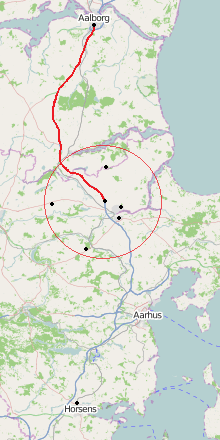
\includegraphics[scale=0.6]{images/AalborgtoHorsens1}  
  \end{center}
\end{frame}

\begin{frame}
  \frametitle{Experiments: The Naive Algorithm}
  \begin{center}
	  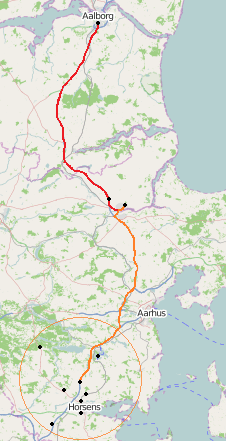
\includegraphics[scale=0.6]{images/AalborgtoHorsens2}  
  \end{center}
\end{frame}

\begin{frame}
  \frametitle{Experiments: The Naive Algorithm}
  \begin{center}
	  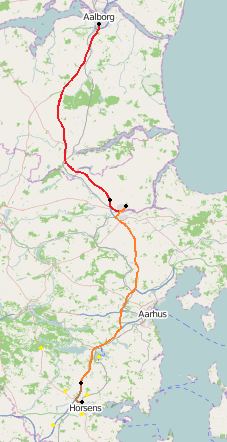
\includegraphics[scale=0.6]{images/AalborgtoHorsens3}  
  \end{center}
\end{frame}

\begin{frame}
  \frametitle{Experiments: Charge station density}
  \begin{center}
	  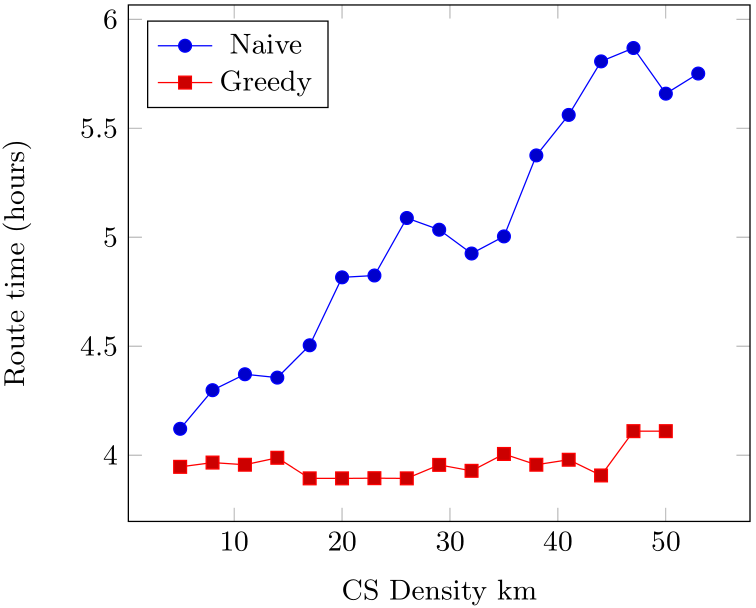
\includegraphics[scale=0.45]{images/CSdensity}  
  \end{center}
\end{frame}

\begin{frame}
  \frametitle{Experiments: Charge station density}
  \begin{columns}[c]
  \column{.5\textwidth} 
  	\begin{center}
  		\begin{figure}
	  	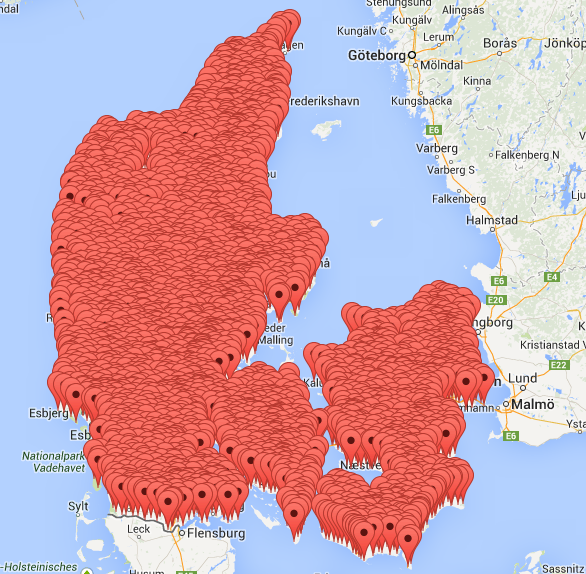
\includegraphics[scale=0.3]{images/density5km}
	  	\caption{5 km between Charge Stations}
	  	\end{figure} 
  	\end{center}
   \column{.5\textwidth}
   \begin{center}
   		\begin{figure}
	  	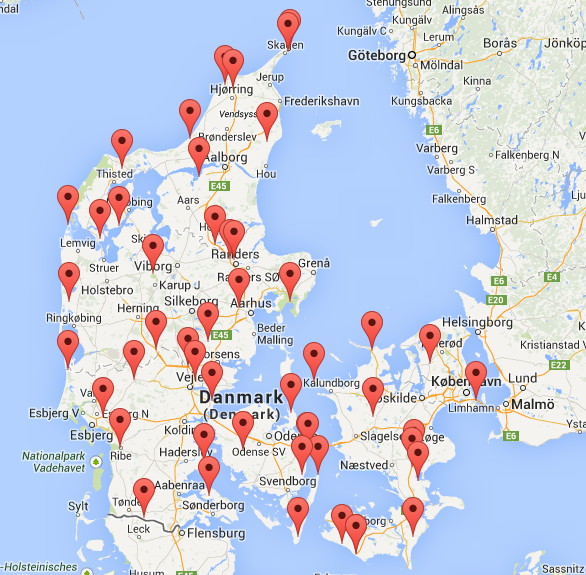
\includegraphics[scale=0.3]{images/density50km} 
	  	\caption{50 km between Charge Stations}
	  	\end{figure}
   \end{center}
   \end{columns} 
\end{frame}

\begin{frame}
  \frametitle{Experiments: Quality Assessment}
  \begin{itemize}
  	\item Standard setup
  	\item Average from 8 experiments
  \end{itemize}
  \vspace{0.8cm}
  {\large Results:}
  \begin{columns}[c]
    \column{.5\textwidth} 
    \begin{center}
    	\begin{tabular}{ | l l |}
    	\textcolor{blue}{Naive} & \textcolor{blue}{$7.461$} \\
    	\textcolor{red}{LP} & \textcolor{red}{$5.684$} \\
    	\end{tabular}
  	\end{center}
    \column{.5\textwidth}
    \begin{center}
    	\begin{tabular}{ | l l |}
    	\textcolor{blue}{Greedy} & \textcolor{blue}{$5.238$} \\
    	\textcolor{red}{LP} & \textcolor{red}{$5.228$} \\
    	\end{tabular}  
    \end{center}
   \end{columns} 
\end{frame}

\begin{frame}
  \frametitle{Conclusion}
  \begin{itemize}
  \item Not influenced much by CS density  
  \item $0.198 \%$ worse than LP
  \item Too slow in practice
  \end{itemize}
\end{frame}


\end{document}
